\chapter{Data Structures}
In this chapter we will briefly introduce the data structure used in the projects.

\section{Graphs}
\subsection{Graphs as matrix of costs}
One way to represent a graph is as a matrix of the costs associated to each edge. node to any other one. This is a generalization of the simpler adjacency matrix, where each cell $a_{ij}$ of the matrix is set to $1$ if there is an edge connecting nodes $i$ and $j$, and $0$ if no edge connects nodes $i$ and $j$. Instead, the cost matrix contains in every cell $c_{i,j}$ the cost associated to the edge connecting nodes $i$ and $j$. If no such edge exists, then the value can be set to $\infty$, or some other conventional value. Such matrix is of course a square one.

If we do not allow the graph to contain self-loops, then the major diagonal will contain the conventional value $0$.

If the graph is undirected, then we do not distinguish from going from node $i$ to node $j$ or the other way around, and therefore $c_{i,j} = c_{j,i}$. Instead, if the graph is directed, those two values may differ.

Representing a graph as a matrix allows a very easy manipulation, since we can accedd directly to every element, by knowing its indexes, but at the cost of a large occupation of memory. Given that we have $|V|$ nodes, we need to store $|V|^2$ values. If we have a complete graph, or a near-complete one, then the matrix of costs is a reasonable choice, since no space will be wasted. If, instead, we are dealing with a sparse graph, an alternative representation like adjacency list may save a lot of space.

\subsubsection{Notes on C implementation}
We provide the \codeline{matrixGraph.h} interface to represent cost matrices. It contains a \codeline{struct} containing:
\begin{itemize}[noitemsep]
  \item the number of nodes;
  \item a list of all the nodes;
  \item a list of all the edges, containing the weight of the edges.
\end{itemize}

The list of edges is thought as a triangular matrix, which is all it is need to know to retrieve the informations for all the edges, since the graph we want to represent is an undirected graph. In figure \ref{fig:costmatrix} we provide a graphical representation of how the memory is managed. Red cells are the ones containing enough information to perform all the operations.

\begin{figure}[hbtp]
  \centering
  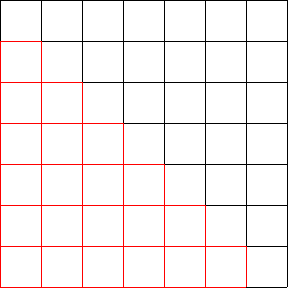
\includegraphics[width=.4\columnwidth]{images/cost_full.png}
  \caption{Graphical representation of the cost matrix.}
  \label{fig:costmatrix}
\end{figure}

The triangular matrix below the main diagonal contains the costs of edges $(1,0)$, $(2,0)$, $(2,1)$, $(3,0)$, \dots, which can be used also for edges $(0,1)$, $(0,2)$, $(1,2)$, $(0,3)$ \dots, while the main diagonal will never be accessed. We can ``unroll'' the matrix in a single list, according to the following property: given two nodes $i$, $j$, $i>j$, the cost of the edge connecting them is stored in $\binom{i}{2}+j = \frac{i \times (i+1)}{2} + j$. Because we are coding in C, we need to rescale the calculation starting from $0$, and thus we will store $\cost(i,j)$ in position $\frac{i \times (i-1)}{2} + j$. Since $\cost(i,j) = \cost(j,i)$, if $i < j$, $\cost(i,j)$ will be contained position $\frac{j \times (j-1)}{2} + i$. With respect to a direct matrix access, this method has the further cost of an \codeline{if} operation and three arithmetical operations, but allows the saving of the data in slightly less than the half of a full matrix size.
